


% ------------------ DOCUMENT SETUP ------------------ 
% The document class defines the document type (report) and sets the font size (10pt)
\documentclass[10pt]{report}
\author{Felipe Santos Almeida}

% Inputs the Document Packages
% ------------------ PACKAGES ------------------ 
% Packages add extra commands and features to your LaTeX document. 
% In here, some of the most common packages for a thesis document have been added 

% LaTeX's float package
\usepackage{float}

% LaTeX's color package
\usepackage{color}

% LaTeX's main math package
\usepackage{amsmath}

% LaTeX's Caption and subcaption packages
\usepackage[format=hang,font=normalsize,labelfont=bf,labelsep=colon,singlelinecheck=off]{caption}
\usepackage{subcaption}

% The graphicx package provides graphics support for adding pictures.
\usepackage{graphicx}

% Longtable allows you to write tables that continue to the next page.
\usepackage{longtable}

% The geometry packages defines the page layout (page dimensions, margins, etc)
\usepackage[a4 paper, top=25mm, bottom=25mm]{geometry}

% Defines the Font of the document, e.g. Arimo font (Check Fonts here: https://tug.org/FontCatalogue/)
\usepackage[sfdefault]{arimo}

% Font encoding
\usepackage[T1]{fontenc}

% This package allows the user to specify the input encoding
\usepackage[utf8]{inputenc}

% This package allows you to add empty pages
\usepackage{emptypage}

% Allows inputs to be imported from a directory
\usepackage{import}

% Provides control over the typography of the Table of Contents, List of Figures and List of Tables
\usepackage{tocloft}

% The setspace package controls the line spacing properties.
\usepackage{setspace}

% Allows the customization of Latex's title styles
\usepackage{titlesec}

% Allows the customization of Latex's table of contents title styles
\usepackage{titletoc}

% The package provides functions that offer alternative ways of implementing some LATEX kernel commands
\usepackage{etoolbox}

% Provides extensive facilities for constructing and controlling headers and footers
\usepackage{fancyhdr} 

% Typographical extensions, namely character protrusion, font expansion, adjustment 
%of interword spacing and additional kerning
\usepackage{microtype}

% Manages hyperlinks 
\usepackage[colorlinks=true,linkcolor=black,urlcolor=blue]{hyperref}

% Generates PDF bookmarks
\usepackage{bookmark}

% Add color to Tables
\usepackage[table,xcdraw]{xcolor}

% Use these two packages together -- they define symbols
%  for e.g. units that you can use in both text and math mode.
\usepackage{gensymb}
\usepackage{textcomp}

% Bibliography package
\usepackage[backend=biber,style=nature]{biblatex}
\addbibresource{references.bib} % Add the .bib file that contains the references

% The natbib package allows book-type citations (e.g. (Saucer et al., 1993))
% More details are here: http://merkel.zoneo.net/Latex/natbib.php
%\usepackage[round]{natbib}

% The linenumbers command adds line numbers next to your text 
% That can be useful for discussing edits in drafts.
%\usepackage[modulo]{lineno}
%\linenumbers 


% This package provides an easy way to input latin sample text (for the template only)
\usepackage{blindtext}


\usepackage{booktabs}

% Controls how many subsections the document can take
%  and how many of those will get put into the contents pages.
\setcounter{secnumdepth}{2}
\setcounter{tocdepth}{2}

% Line Spacing
\setstretch{1.0}

% The folder path where the images will be uploaded
\graphicspath{{./Images/}} 

% Places a dot after Chapter/Section/Subsection number in Table of Contents
\renewcommand{\cftchapaftersnum}{.}
\renewcommand{\cftsecaftersnum}{.}
\renewcommand{\cftsubsecaftersnum}{.}

%  Customize Dot spacing in Table of Contents/List of Figures/Tables
\renewcommand{\cftdotsep}{0.3}

% Numeration Type for Chapters and Sections (Roman I, II, II / Arabic 1, 2, 3)
\renewcommand\thechapter{\Roman{chapter}}
\renewcommand\thesection{\arabic{section}}

% Line Break Properties
\tolerance=1
\emergencystretch=\maxdimen
\hyphenpenalty=10000
\hbadness=10000


% Formatting Table of Contents/Lists titles
\renewcommand{\contentsname}{\normalfont\bfseries\LARGE{CONTENTS}}
\renewcommand{\listfigurename}{\normalfont\bfseries\LARGE{LIST OF FIGURES}}
\renewcommand{\listtablename}{\normalfont\bfseries\LARGE{LIST OF TABLES}}


% Title Formatting customization
\titleformat{\chapter}{\normalfont\bfseries\LARGE}{\thechapter.}{1em}{\MakeUppercase}

\titleformat{\section}{\normalfont\bfseries\large}{\thesection.}{1em}{\MakeUppercase}
\titlespacing*{\section} {0pt} {0pt} {15pt} % left, before, after

\titleformat{\subsection}{\normalfont\bfseries\large}{\thesubsection.}{1em}{}
\titlespacing*{\subsection} {0pt} {10pt} {10pt}

\titleformat{\subsubsection}{\normalfont\bfseries\large}{}{1em}{}
\titlespacing*{\subsubsection} {0pt} {10pt} {10pt}


% HEADER AND FOOTER
\pagestyle{fancy}  % Set Page Style (Header and Footer Style)
\fancyhf{}  % Clears the header and footer (from the default info)

% Header
\renewcommand{\headrulewidth}{0pt}  % Removes the default Horizontal Line in Header
\fancyhead[L]{SN21125032}
\fancyhead[R]{May 2023}

% Footer
\fancyfoot[C]{\thepage} % Page Number

% Change figure numbering per section
\numberwithin{figure}{section}
\numberwithin{table}{section}






%  -------------------------------------------------
%  --------- The document starts from here --------- 
%  -------------------------------------------------

\begin{document}

% -------------------  INTRODUCTION  ---------------------

\begin{center}
    % UCL IMAGE
    \vspace*{-3cm}
    \makebox[\textwidth]{
\includegraphics[width=\paperwidth]{Image/UCL_LOGO_new.png}}
\end{center}   
    % Title
    {\LARGE\textbf{Assessment\\
    % Subtitle
    CASA0002 – Urban Simulation\\}}
    

\section{Part 1: London’s underground resilience}


 \subsection{Topological Network}
\subsubsection{Centrality Measures } 
        
         Aiming to evaluate the resilience of the Tube Network and the impact of node removals, the three centralities measures chosen to identify the most important nodes in the Tube Network are Degree, Eigenvector, and Betweenness centrality. In the first experiment of this analysis was also considered to use closeness centrality. However, the application in the context of nodes removal this centrality measure not presented good results.  
        
        \vspace{5mm} %5mm vertical space
        
        \textbf{Degree Centrality:} The number of links associated with a node related to the tube network. This centrality reflects the number of connections with a station, which can be linked with another station or tube line that starts and finish in the same station, as a loop, for example. Regarding this analysis, the degree centrality values are normalised by dividing them by the maximum possible degree, which is n-1. 

    \begin{figure}[htp]
        \centering
        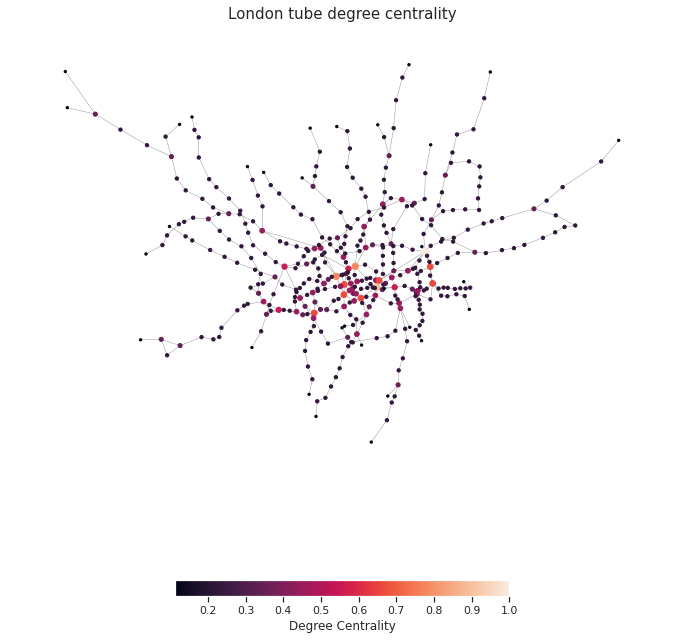
\includegraphics[width=14cm]{Image/Part1_topologicalmap_degree.png}
        \caption{Topological Tube network map - Degree centrality}
        \label{fig:galaxy}
    \end{figure}   


        
  \vspace{5mm} %5mm vertical space
        
        \textbf{Eigenvector centrality:}  The transitive influence of nodes. Eigenvector centrality measures the influence of a node in a network based on a relative score for all nodes. Thus, nodes with a high-score mean that these nodes are also connected to other nodes with a high score. For tube network, these measure is useful because it is possible to understand the influence of a tube station not only focused on its good connectivity with a  range of tube lines. This centrality allows us to understand how good is the connectivity of the neighbour's stations. Therefore, when it is considered a station disruption, an individual close to other stations is well-connected to improve the user experience in the system. 

        
    \begin{figure}[htp]
        \centering
        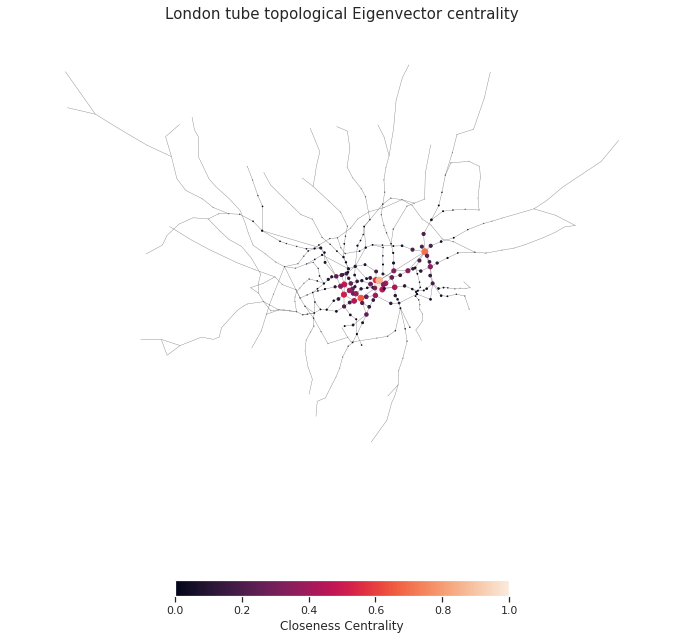
\includegraphics[width=14cm]{Image/Part1_topologicalmap_eigenvector.png}
        \caption{Topological Tube network map - Eigenvector centrality}
        \label{fig:galaxy}
    \end{figure} 

   \vspace{5mm} %5mm vertical space
   
        \textbf{Betweenness centrality:} the shortest path passing through a node.
        
    \begin{figure}[htp]
        \centering
        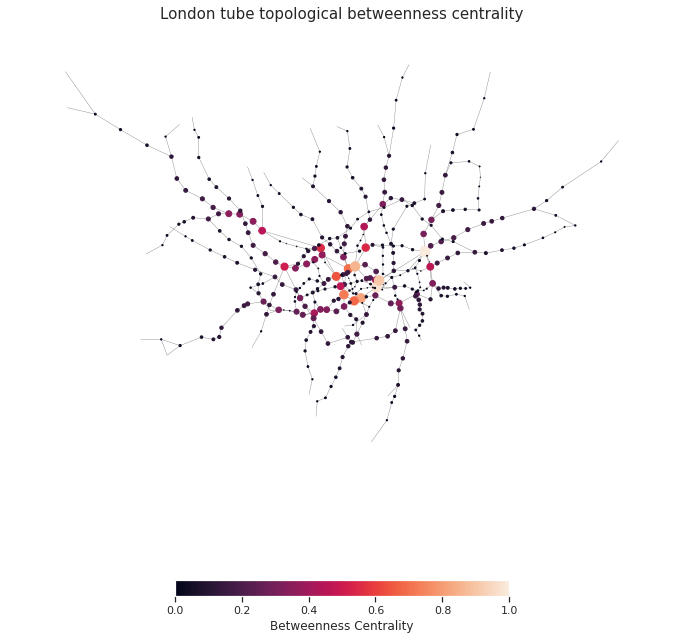
\includegraphics[width=14cm]{Image/Part1_topologicalmap_betweenness.png}
        \caption{Topological Tube network map - Betweenness centrality}
        \label{fig:galaxy}
    \end{figure} 


    To summarise,     

    \begin{figure}[htp]
        \centering
        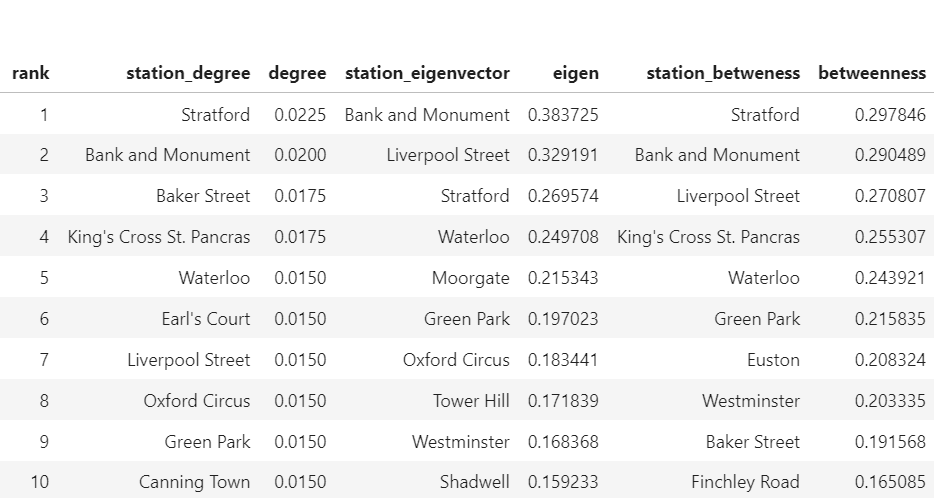
\includegraphics[width=14cm]{Image/Table_CentralitiesMeasures.png}
        \caption{Centrality measures}
        \label{fig:galaxy}
    \end{figure}

\newpage    

\subsubsection{Impact Measures} 

In order to evaluate the topological network and use this measure to evaluate the removal of stations, this analysis uses [measure 1] and [measure 2]. The current network has only 1 component. However, when the stations start to be removed, some links will be disconnected, and the number of components will increase. Thus, it is crucial to choose measures that can detect the impact of removing that station, considering the rearrangement of the topological network. 

\subsubsection{Node Removal} 

    \begin{figure}[htp]
        \centering
        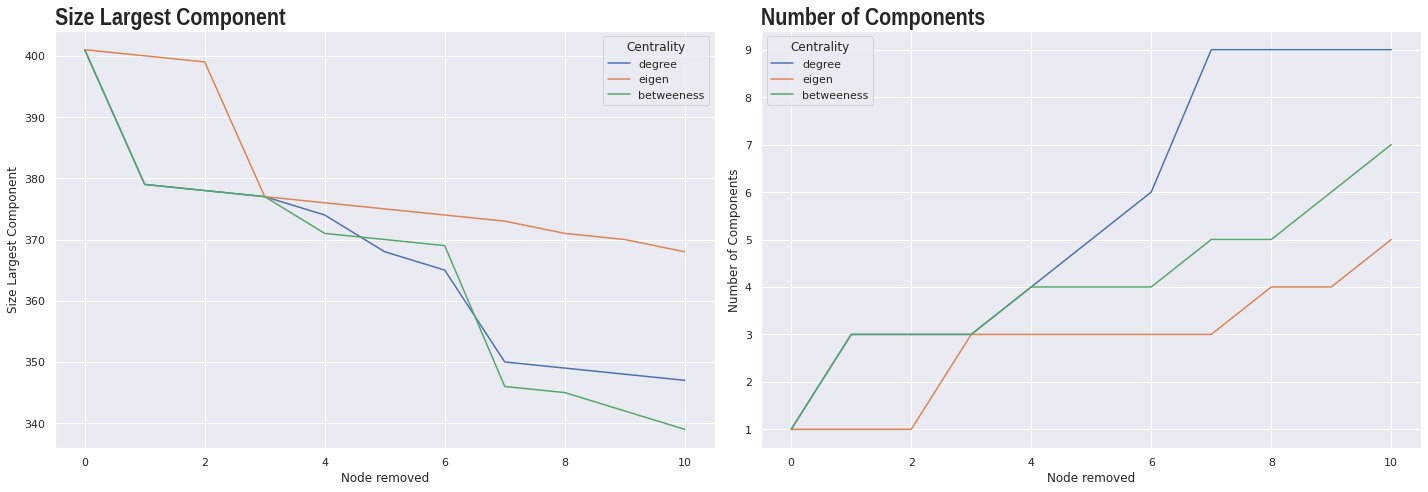
\includegraphics[width=16cm]{Image/Part1_nonsequential_Summarise.png}
        \caption{Non-sequential node removal}
        \label{fig:galaxy}
    \end{figure}


    \begin{figure}[htp]
        \centering
        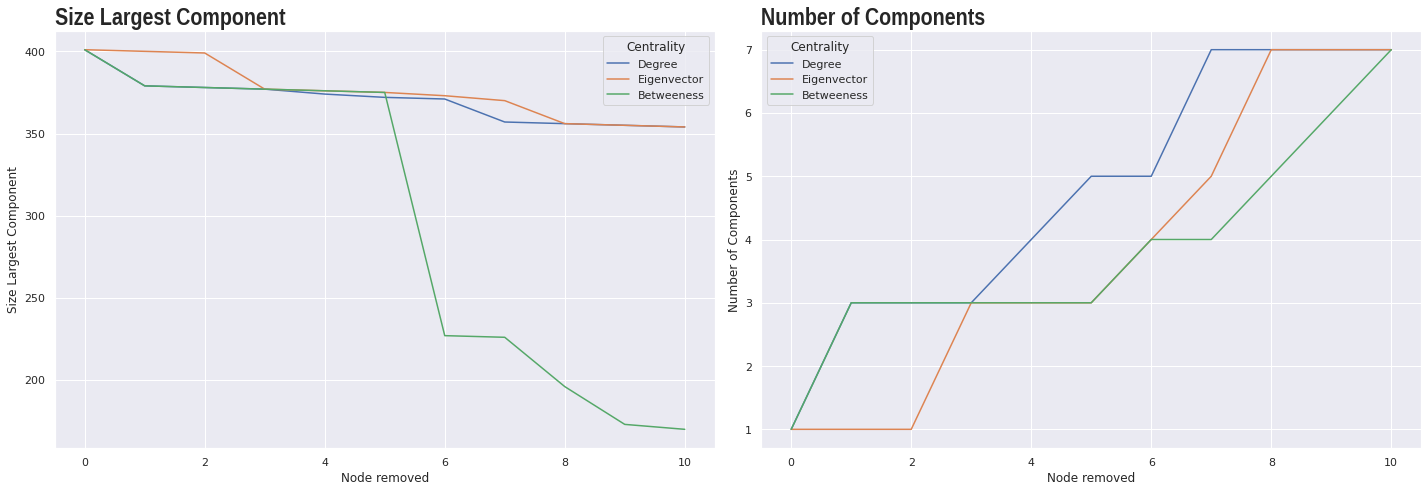
\includegraphics[width=16cm]{Image/Part1_sequential_Summarise.png}
        \caption{Sequential node removal}
        \label{fig:galaxy}
    \end{figure}


\newpage

\subsection{Flows: weighted network} 

\subsubsection{Centrality Measures } 

    \begin{figure}[htp]
        \centering
        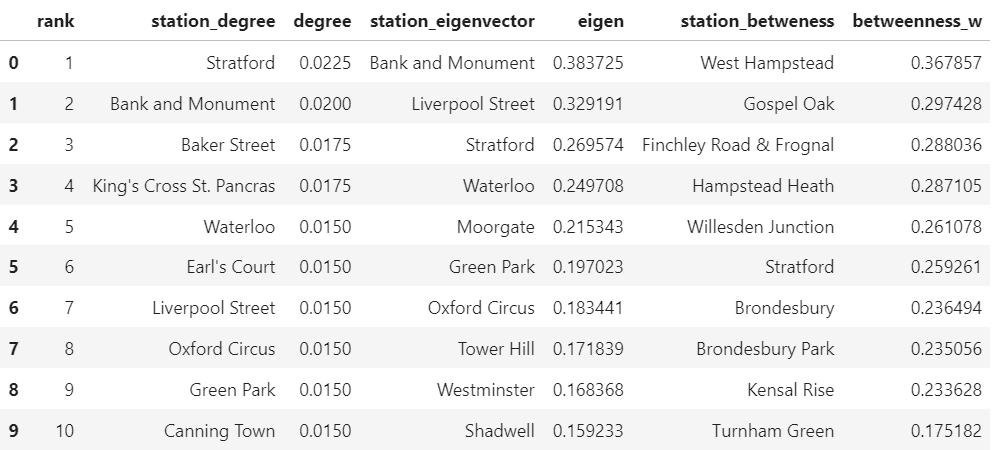
\includegraphics[width=14cm]{Image/Table_CentralitiesMeasures_Flows.png}
        \caption{Flows - Centrality measures}
        \label{fig:galaxy}
    \end{figure}


\subsubsection{Impact Measures} 
lorem

\subsubsection{Node Removal} 

    \begin{figure}[htp]
        \centering
        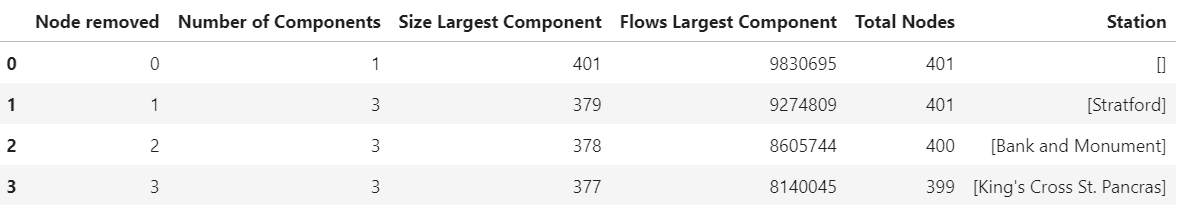
\includegraphics[width=14cm]{Image/Table_Flows_degree.png}
        \caption{Flows - Centrality measures}
        \label{fig:galaxy}
    \end{figure}

    \begin{figure}[htp]
        \centering
        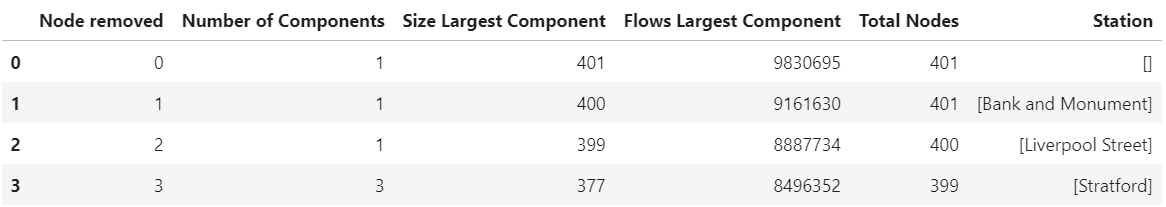
\includegraphics[width=14cm]{Image/Table_Flows_eigenvector.png}
        \caption{Flows - Centrality measures}
        \label{fig:galaxy}
    \end{figure}


    \begin{figure}[htp]
        \centering
        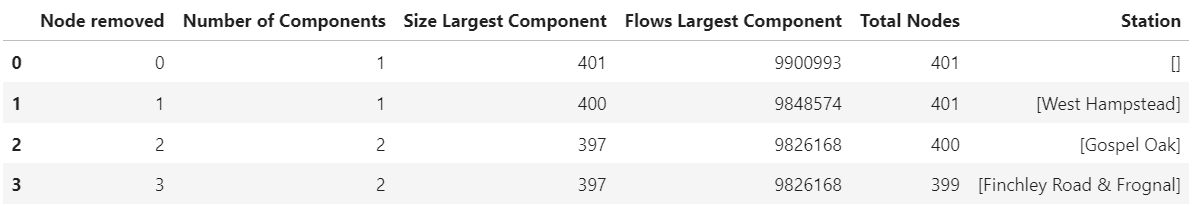
\includegraphics[width=14cm]{Image/Table_Flows_Betweenness.png}
        \caption{Flows - Centrality measures}
        \label{fig:galaxy}
    \end{figure}

\newpage

\section{ Part 2: Spatial Interaction models}


\subsection{Models and calibration}







    \begin{figure}[htp]
        \centering
        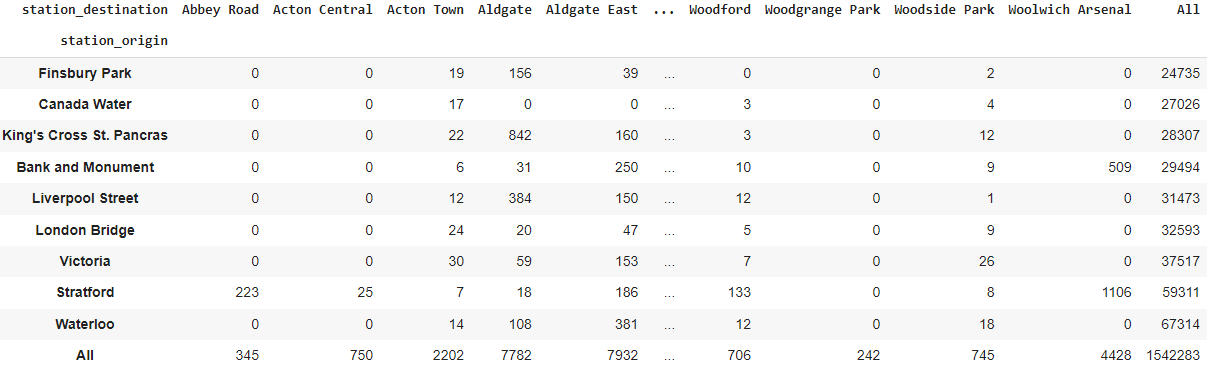
\includegraphics[width=16cm]{Image/Part2_OD.png}
        \caption{Table}
        \label{fig:galaxy}
    \end{figure}

    \begin{figure}[htp]
        \centering
        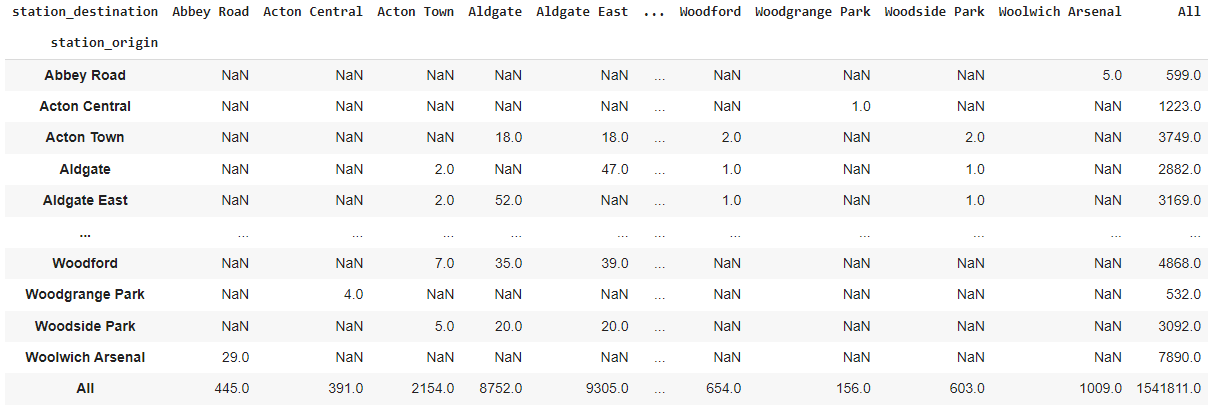
\includegraphics[width=16cm]{Image/Part2_OD2.png}
        \caption{Table}
        \label{fig:galaxy}
    \end{figure}

\newpage    
\subsection{Scenarios}
\subsubsection{Scenario A}

    \begin{figure}[htp]
        \centering
        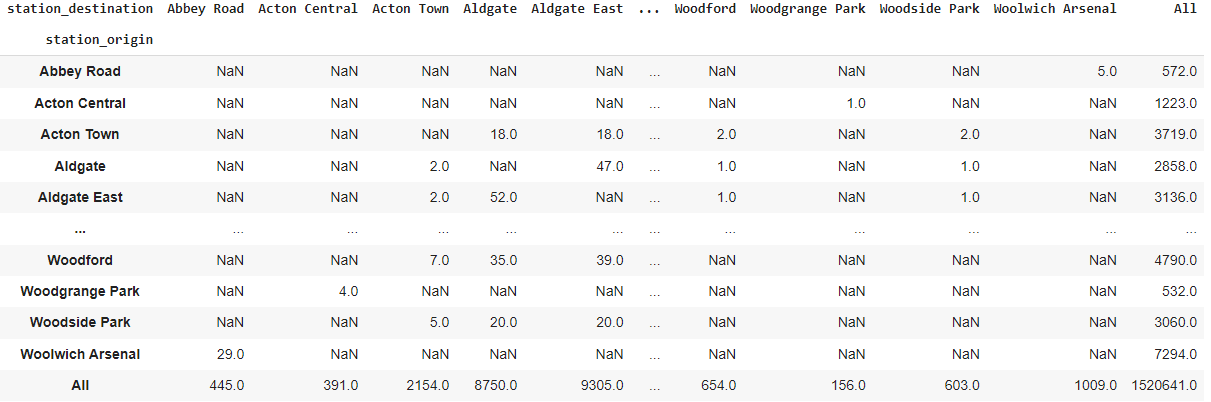
\includegraphics[width=16cm]{Image/Part2_OD3_scenario A.png}
        \caption{Table}
        \label{fig:galaxy}
    \end{figure}

    \begin{figure}[htp]
        \centering
        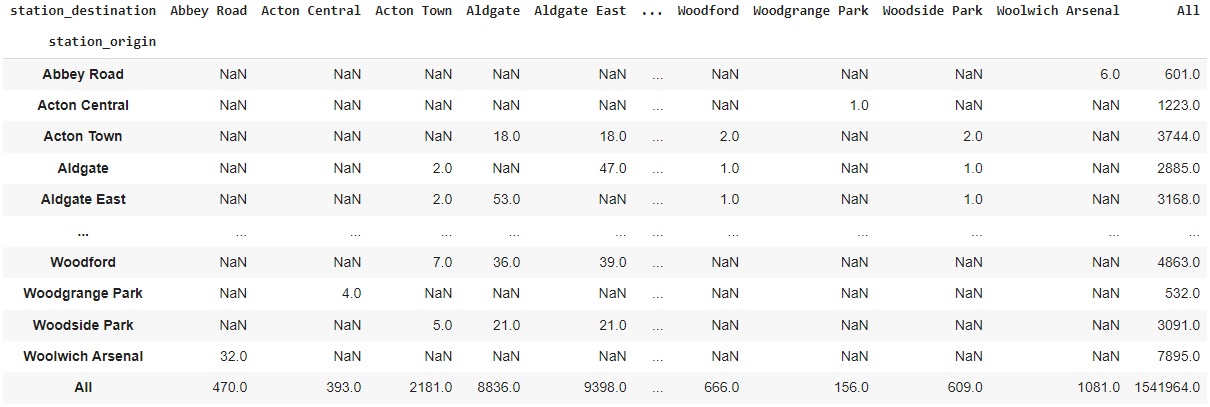
\includegraphics[width=16cm]{Image/Part2_OD4_scenario A.png}
        \caption{Table}
        \label{fig:galaxy}
    \end{figure}

\newpage    

\subsubsection{Scenario B}

\textbf{Measure 1}
    \begin{figure}[htp]
        \centering
        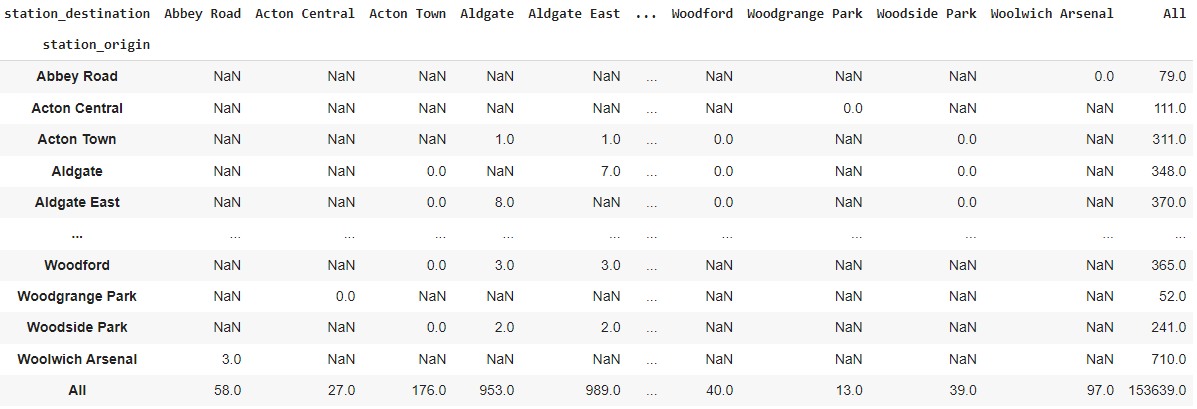
\includegraphics[width=16cm]{Image/Part2_OD5_scenario B.png}
        \caption{Table}
        \label{fig:galaxy}
    \end{figure}

    \begin{figure}[htp]
        \centering
        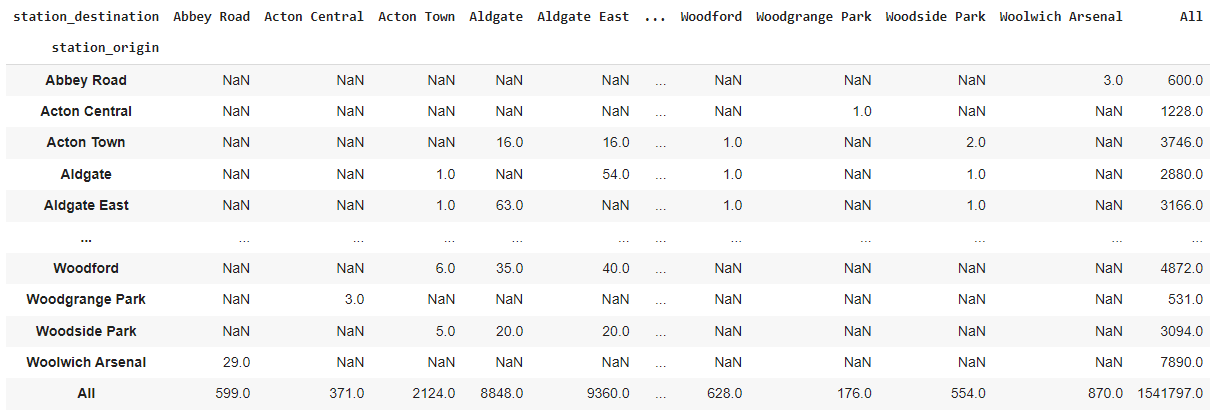
\includegraphics[width=16cm]{Image/Part2_OD6_scenario B.png}
        \caption{Table}
        \label{fig:galaxy}
    \end{figure}

\textbf{Measure 2}    
    \begin{figure}[htp]
        \centering
        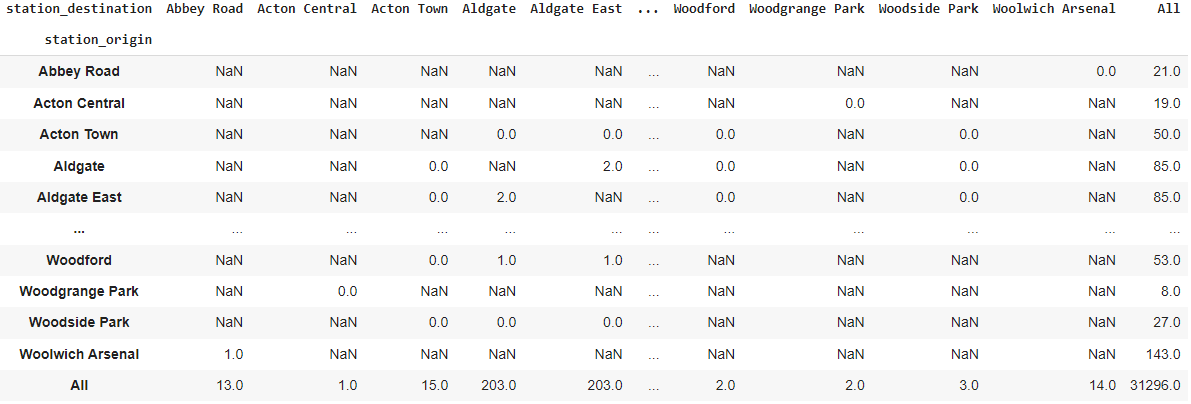
\includegraphics[width=16cm]{Image/Part2_OD7_scenario B.png}
        \caption{Table}
        \label{fig:galaxy}
    \end{figure}

    \begin{figure}[htp]
        \centering
        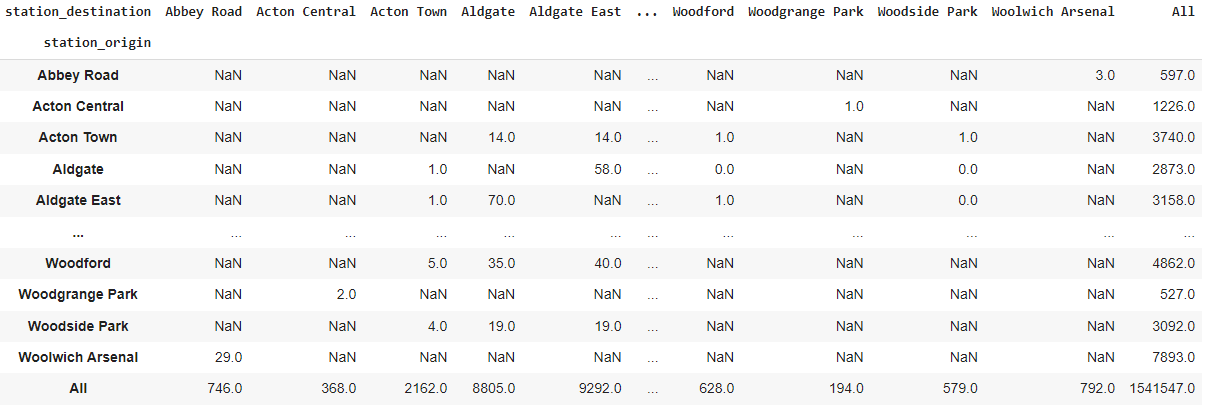
\includegraphics[width=16cm]{Image/Part2_OD8_scenario B.png}
        \caption{Table}
        \label{fig:galaxy}
    \end{figure}

\newpage    

\subsubsection{Discussion}













% -------------------  BIBLIOGRAPHY ---------------------
\newpage
\printbibliography[title = {References}]
\addcontentsline{toc}{chapter}{References} % Adds References Section to Table of Contents


\end{document}
%  -------------------------------------------------
%  --------- The document ends from here ----------- 
%  -------------------------------------------------